\documentclass[12pt,a4paper,oneside]{article}
\usepackage{times}
\usepackage{graphicx}
\usepackage{hyperref}
\usepackage{setspace}
\usepackage{fixltx2e}
\usepackage{amsmath}
\usepackage{apacite}
	
\begin{document} 
\bibliographystyle{apacite}

\begin{titlepage}
	\null \vfill
   \begin{center}
    {\LARGE \textbf{Research Proposal}}
			\vspace{20mm}
			
			
			
			{\Large  \textbf{A System for Real Time Image Processing \\for 
            	\\Vehicle Detection, Indexing, Searching, and Tracking using 						Synchronized Video Data \\from \\UAV (Unmanned Aerial Vehicle)  and 				Traditional Traffic Cameras \\for \\Urban Traffic Surveillance }}
			\vspace{8mm}
			
			
   \end{center}
  	\vfill
		\vfill
		
		\begin{flushright}
			
			\textbf{Document Date :}\\
			\today
			\vspace{7mm}
			
			\textbf{Prepared for :}\\
            {\large John See Su Yang\\}
            TPT1201 Research Methodology in CS\\
            Lecture: TC01 Tutorial: TT02\\ 
            Multimedia University 
			\vspace{7mm}
			
			\textbf{Authors :}\\
			{\large Mahmood Sarzil 1141126473 \\
			 \large Meheraj Akhter Anika 1151301799 \\}
			
			
			
		\end{flushright}
		\hfill
			
		
\end{titlepage}
\tableofcontents
\newpage

\null
\section{Executive Summary of Research Proposal}

Traffic cameras normally are modern day needs which are mostly maintained by state traffic surveillance department. To get valuable data for making influential decisions, aid commuters, enforce law, encourage safe driving etc. are part of the equation. But accuracy and integrity must be guaranteed in quality when the real time concept comes in, otherwise the inaccuracies can lead from minor to complicated problems that demolishes the work and effort. This is where our goal for developing the system comes, its Real time image processing for Vehicle detection, indexing, searching, and tracking using synchronized video data from UAV and traditional traffic cameras for Urban traffic surveillance. Bird’s eye view, live surveillance, background processing and creating constructive algorithm were the main functionality of this system. It can find relative temporal offsets of clips from a camera array to construct a video panorama without ghosting on moving objects. Background elimination gives a more solid result for detection and tracking. Vehicle symmetric attributes are indexed in database for machine learning to automate the process as it provides a vehicle search system. Our system aims for accuracy and precision for the surveillance system by eliminating the disturbance around the subject area as well as synchronizing the data collected.


\newpage
\section{Introduction}

Live and detailed information about traffic condition is very important for urban traffic control department. Various devices and systems have been used to get timely feedback for urban traffic surveillance. Many Traffic control departments around the world is using modern Real time image processing for traffic surveillance using devices like surveillance video camera, UAV (Unmanned Aerial Vehicle) etc. The system proposed in this report differs from the other system in the term 'Synchronization'. 

The system is proposed to be developed as a real time image processor using video data not only from traffic camera or UAV but synchronizing the data achieved from both devices. After being processed to eliminate background disturbance such as shadow, reflection, glare etc the system detects and identifies and detects vehicles, indexes their symmetric attributes, searches desired vehicles and tracks their path. Thus giving live and valuable informations such as direction of travel, vehicle attributes etc to the traffic control department or law enforcing department for better control over traffic conditions and criminal tracking.   

\section{Justification/Motivation of the Research Problem}
Traditionally, when one speaks about urban traffic surveillance, one is referring to the urban traffic light management and perhaps a little bit on crowd surveillance. But Traffic surveillance is much more than these. As stated in \cite{puri2005survey} “The United States Department of Transportation (DOT) has been interested for the past several years in obtaining data on traffic trends and to monitor and control traffic in real time. Currently, there are several methods by which the DOT regulates and monitors road transport. Cameras mounted on towers, detectors embedded in pavements or pneumatic tubes, and unmanned aircraft have been proven to be expensive and time-consuming solution candidates. However, aerial monitoring has the potential to yield detailed information to help traffic planners, as well as commuters. Unmanned Aerial Vehicles (UAVs) may provide a “bird’s eye view” for traffic surveillance, road conditions and emergency response.” But we think that video data provided from UAVs only is not enough for a flawless traffic surveillance system. 
So the motivation behind this research problem is to ensure a system that provides live 24/7 surveillance on traffic and able to detect and track vehicles using real time video image processing by synchronized video data collection from both traffic cameras and UAV. Thus ensuring a easier and precise traffic surveillance system. 

\section{Research Objectives}

\subsection{Overall Objectives}

\begin{itemize}
\item To provide urban traffic control department the ability to survey traffic conditions with ease and precision. 
\item The system can be used to detect and track desired vehicles with the help of synchronized real time video data from both traffic cameras and UAVs thus ensuring faster and more accurate results than most other surveillance systems available. 

\item By providing relevant and convenient data, the system will be able to help the law enforcement departments to track criminals and also control emergency urban traffic situations.
\end{itemize}
\subsection{Specific Objectives}
\begin{itemize}
\item Using real time image processing on video data, the system is able to provide 24/7 live traffic surveillance.

\item Synchronized video data from both traffic cameras and UAVs provides a wider angle of view on the traffic condition to sift out accurate symmetric attributes of vehicle objects. 

\item Background image processing in real time enables better vehicle detection from live video by eradicating background disturbance.

\item The  system is able to detect and then track the patch of any designated vehicles in the area of surveillance. 

\item The system is able to index symmetric attributes of different vehicles to form a learning algorithm for faster search mechanism.

\item The 'bird's-eye' view from UAVs and the layout view from traffic cameras will sync to provide a real time simulation of traffic conditions for better traffic management.
\end{itemize}

\newpage
\null
\section{Literature Review}

Designated system for better traffic surveillance has been attracting interest of researchers for a long time period. A lot of researches has been done so far, relating UAV traffic surveillance or Real time image processing for vehicle detection. These prior researches can be both explicitly/implicitly related for the purpose of creating the structure of this system. 

In a research paper, prepared for Florida Department of Transport \cite{farradine2005use} , the authors have established a concept on UAV traffic surveillance system that can be used as an architectural component for UAV operation for the proposed system. There are other research papers which discuss traffic surveillance system using UAV E.g. The research paper of \cite{srinivasan2004airborne} has described a system of Airborne traffic surveillance for highway traffic monitoring, the system can respond to emergency traffic conditions. In another research \cite{puri2007statistical} the authors have established a system that is able to generate statistical profile for traffic monitoring in an area using video data from multiple UAVs. 

For real time vehicle detection it is immensely necessary to understand \cite{viola2001robust} research on robust object detection. Viola-Jones object detection algorithm can be used and evolved to detect Large scale vehicle from traffic scene. To eradicate background disturbance for vehicle detection while using traditional traffic cameras, \cite{feris2012large} was able to pursue a system for Large scale vehicle detection. Another paper \cite{cucchiara2001improving} describes method for improving shadow suppression in moving object detection, which can be used to solve the issue while tracking vehicle objects. For better detection mechanism smart camera system described in the research of \cite{bramberger2003smart}, is affordable in exchange for better image quality from real time video data. Data fusion algorithms provided in ‘A Handbook of Algorithm- Tracking and Data Fusion’ \cite{bar2011tracking} can be evolved to be used for synchronized video data collection from multiple image sensors of UAVs and traffic cameras. 

\newpage
\section{Research Methodology}
The system proposed in this research is able to perform multiple tasks in order to provide an enhanced system for traffic surveillance. Brief description on estimated methodology to be adopted to carry out the research for the system is described further. 

\subsection{Synchronizing Video Data}

A multi camera synchronizing system described in \cite{wang2014videosnapping} can be evolved and used for the purpose of synchronizing constant video data input from both UAV cameras and traditional mounted traffic cameras. A fine example of multiple video source input synchronization is shown in Fig.1 for better understanding :

\begin{center}
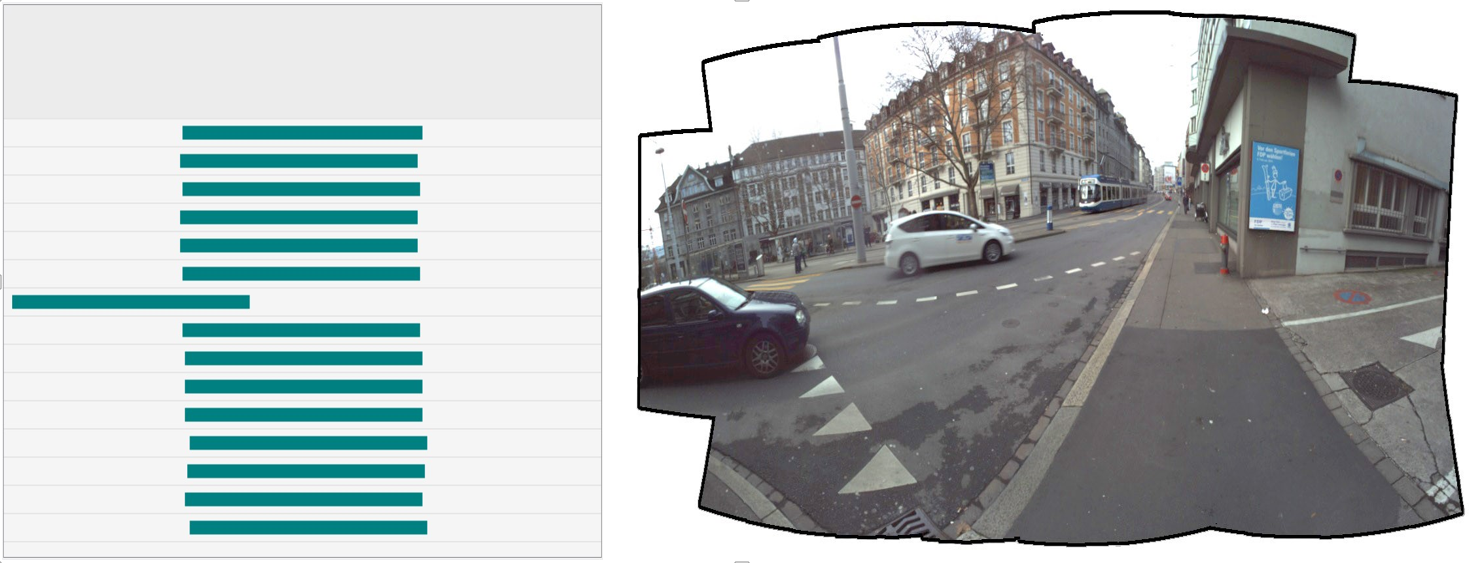
\includegraphics[width=0.8\linewidth]{Fig1.PNG}\\
Fig.1 : By finding relative temporal offsets of clips from a 15 camera array (left), it becomes possible to construct a video panorama without ghosting on moving objects (right)
\end{center}

\subsection{Real Time Image Processing to eradicate background disturbance}

After being synchronized, video data from both parameters will go through a process in real time to extract background disturbances such as: shadow, reflection, occlusion, glare etc. To achieve this task several prior researches can be used and evolved. E.g. in the research paper of \cite{feris2012large}, a promising system to eradicate this problem for Traffic cameras is shown. This system has the potential to be evolved for UAV’s video data collection. Though UAVs face little less difficulties than traditional cameras mounted on roads. 

\newpage
\subsection{Vehicle Detection and Tracking}

Vehicles from video data can be simplified as objects and thus can be detect using several layered method. Methods described in researches like \cite{viola2001robust}, \cite{cucchiara2001improving} etc for object detection can be used to detect moving vehicles from synced video data. An example of successful vehicle detection and tracking is shown in Fig.2 :

\begin{center}
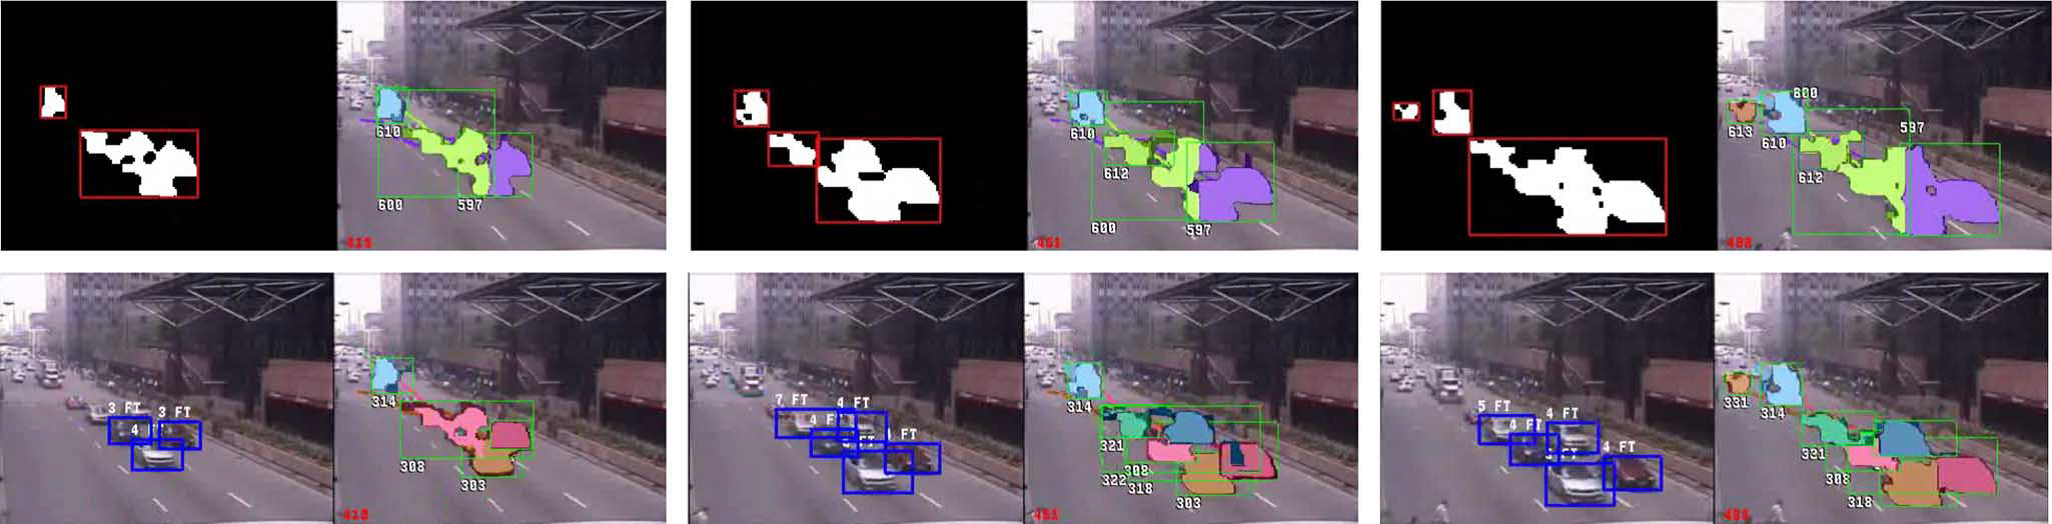
\includegraphics[width=0.8\linewidth]{Fig2.png}\\
Fig. 2: Tracking Results: Top row-tracking results for three non-consecutive frames of an image sequence where the left picture in each frame shows the result of background subtraction and the right picture shows tracking results using only background subtraction. Bottom row-left picture in each frame shows result of vehicle detection and the right picture in each frame shows tracking results using both the background subtraction and the detection results. Note that the inclusion of detection results allows us to perform tracking at a higher fidelity.
\end{center}

\subsection{Vehicle Indexing and Search}

Vehicle symmetric attributes are constantly indexed in database for machine learning. The goal is to automate this process by providing a vehicle search system based on semantic attributes. The implementation will allows the user to search for vehicles based on color, size, length, width, height, speed, direction of travel, date/time, and location, and many more attributes could be considered.  

\newpage
\bibliography{Bibpaper.bib}
\end{document}
